\documentclass{article}
\usepackage{amsmath}
\usepackage{hyperref}
\usepackage{graphicx}
\usepackage{float}
\usepackage[top=2cm]{geometry}

\title{Deep Learning - Homework 1}
\author{99222 - Frederico Silva, 99326 - Sebastião Carvalho}
\date{\today}

\begin{document}

\maketitle

\tableofcontents

\section{Question 1}

Medical image classification with linear classifiers and neural networks.

\subsection{Question 1.1}

\subsubsection{Question 1.1 a)}

\paragraph{Answer} After running the code, the following plot was generated:
\begin{figure}[H]
    \centering
    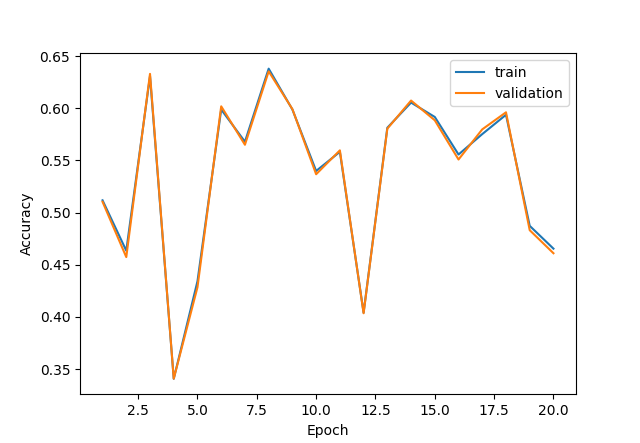
\includegraphics[width=0.8\textwidth]{"plots/1_1_a.png"}
    \caption{Perceptron Training and Validation Accuracy}
    \label{1.1.a Plot}
\end{figure}

The final test accuracy was 0.3422.

\subsubsection{Question 1.1 b)}
\paragraph{Answer} After running the code, the following plots were generated for learning rates $\eta = 0.01$ and $\eta = 0.001$, respectively:
\begin{figure}[H]
    \centering
    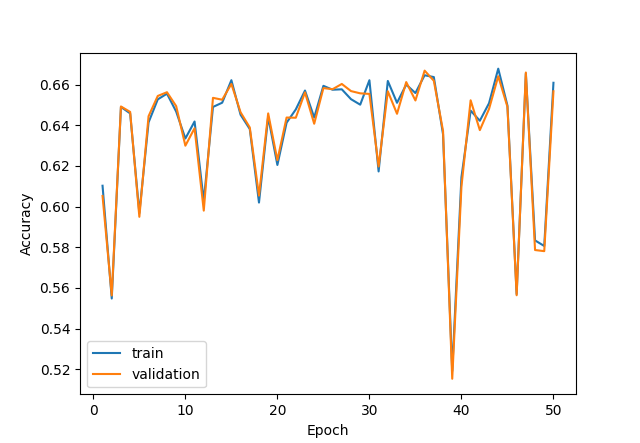
\includegraphics[width=0.8\textwidth]{"plots/1_1_b_001.png"}
    \caption{Logistic Regression Accuracy with Learning Rate $\eta = 0.01$}
    \label{1.1.b 0.01 Plot}
\end{figure}

\begin{figure}[H]
    \centering
    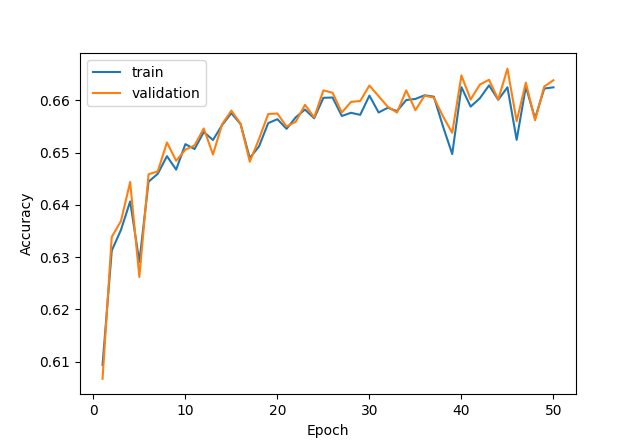
\includegraphics[width=0.8\textwidth]{"plots/1_1_b_0001.png"}
    \caption{Logistic Regression Accuracy with Learning Rate $\eta= 0.001$}
    \label{1.1.b 0.0001 Plot}
\end{figure}

The final test accuracy was 0.5784 and 0.5936 for $\eta = 0.01$ and $\eta = 0.001$ respectively.\\
Comparing both charts, we can see that for $\eta = 0.001$, the accuracy increases more slowly, but it reaches a higher value than for $\eta = 0.01$. 
This is because for $\eta = 0.01$, the algorithm is taking too big steps, and it is not able to converge to a better solution. This can be 
seen in the chart for $\eta = 0.01$, near epoch 40, when the accuracy drops to an all time low.\\
Since the learning rate is too small for $\eta = 0.001$, the algorithm takes longer to reach higher accuracies, but it's also 
less oscillatory, and it is able to converge to a better solution.\\

\subsection{Question 1.2}

\subsubsection{Question 1.2 a)}

\paragraph{Answer}
The answer to this question mainly focus on two topics: how complex the models are, meaning their expressiveness, and how easy they are to train. \\
Regarding the expressiveness, logistic regression is a linear model that learns a single decision boundary to separate classes. 
When using pixel values as features, it treats each pixel independently and cannot capture complex patterns such as shapes or textures 
that might be essential for tasks like image classification.\\ 
On the other hand, a multi-layer perceptron can learn non-linear decision boundaries due to its hidden layers and non-linear activation functions like ReLU. 
Each layer can transform the feature space in a way that makes the data linearly separable by subsequent layers, allowing the MLP to capture 
complex patterns and relationships in the data.\\
When it comes to how easy it is to train this models, logistic regression, with its convex cost function, offers a straightforward training guaranteed 
to reach the global minimum, given enough time and proper learning hyperparameters. 
However, when talking of a multi-layer perceptron, the presence of multiple layers and non-linearities in an MLP makes the optimization landscape non-convex. 
There can be multiple local minima, saddle points, and plateaus. Finding the global minimum is not guaranteed, making the training process, 
most of the times, more complex.\\
In short, the claim is true. A logistic regression model is less expressive than a multi-layer perceptron with ReLU activations because it can only 
represent linear relationships, whereas MLPs can capture non-linearities. Logistic regression models are easier to train because they involve 
convex optimization, unlike the non-convex problem of training MLPs.

\subsubsection{Question 1.2 b)}
\paragraph{Answer} After running the code, the following plots was generated:
\begin{figure}[H]
    \centering
    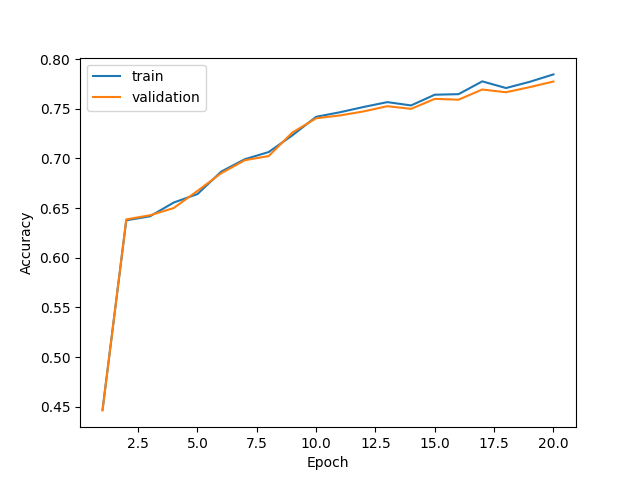
\includegraphics[width=0.8\textwidth]{"plots/mlp_validation_training.png"}
    \caption{MLP Accuracy with Learning Rate $\eta= 0.001$}
    \label{1.2.b 0.001 Plot}
\end{figure}


\begin{figure}[H]
    \centering
    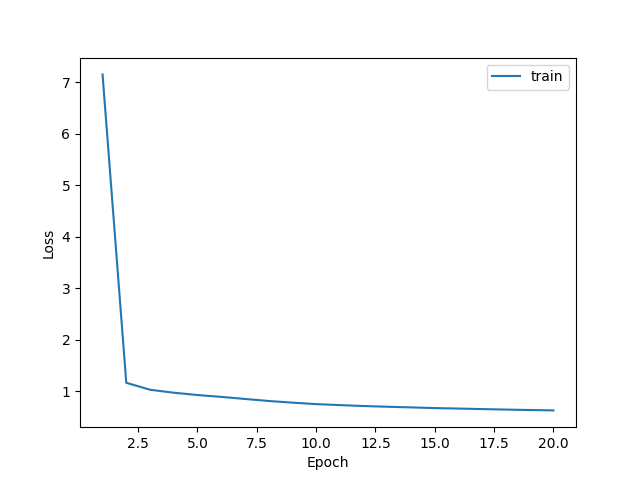
\includegraphics[width=0.8\textwidth]{"plots/mlp_loss.png"}
    \caption{MLP Loss with Learning Rate $\eta= 0.001$}
    \label{1.2.b Loss Plot}
\end{figure}

The final test accuracy was 0.7505.

\section{Question 2}
Medical image classification with an autodiff toolkit.

\subsection{Question 2.1}

\paragraph{Answer} After running the code, the following plots were generated:

\begin{figure}[H]
    \centering
    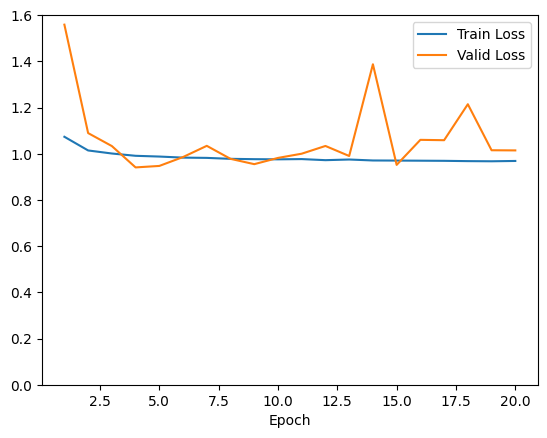
\includegraphics[width=0.8\textwidth]{"plots/logistic_regression-training-loss-batch-16-lr-0.1-epochs-20-l2-0-opt-sgd.png"}
    \caption{Training and validation loss for $\eta = 0.1$}
    \label{2.1 0.1 Loss Plot}
\end{figure}

\begin{figure}[H]
    \centering
    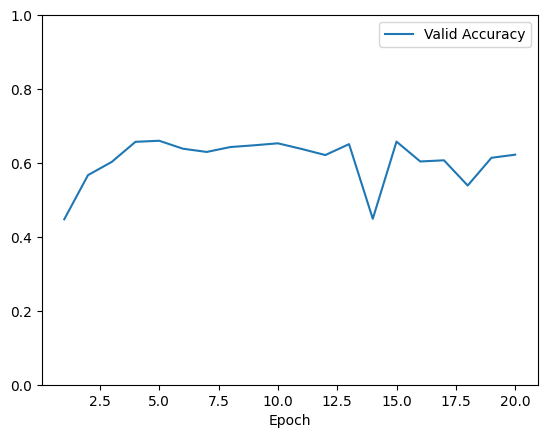
\includegraphics[width=0.8\textwidth]{"plots/logistic_regression-validation-accuracy-batch-16-lr-0.1-epochs-20-l2-0-opt-sgd.png"}
    \caption{Validation accuracy for $\eta = 0.1$}
    \label{2.1 0.1 Acc Plot}
\end{figure}

\begin{figure}[H]
    \centering
    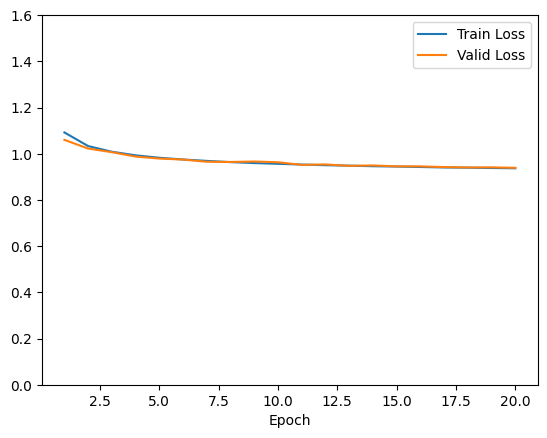
\includegraphics[width=0.8\textwidth]{"plots/logistic_regression-training-loss-batch-16-lr-0.01-epochs-20-l2-0-opt-sgd.png"}
    \caption{Training and validation loss for $\eta = 0.01$}
    \label{2.1 0.01 Loss Plot}
\end{figure}

\begin{figure}[H]
    \centering
    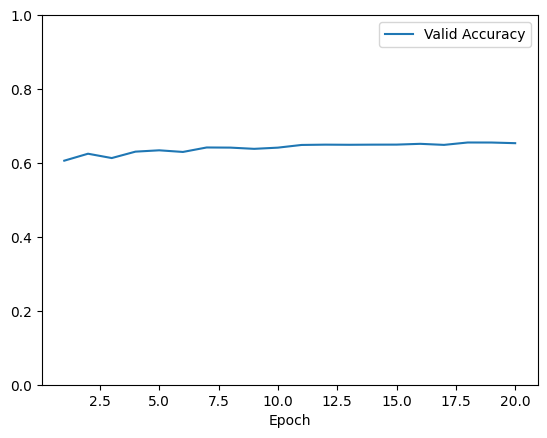
\includegraphics[width=0.8\textwidth]{"plots/logistic_regression-validation-accuracy-batch-16-lr-0.01-epochs-20-l2-0-opt-sgd.png"}
    \caption{Validation accuracy for $\eta = 0.01$}
    \label{2.1 0.01 Acc Plot}
\end{figure}

\begin{figure}[H]
    \centering
    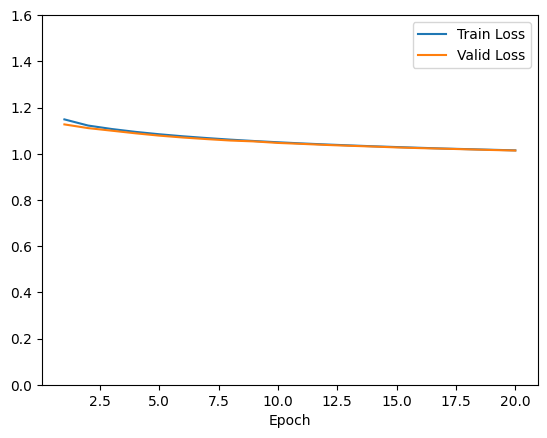
\includegraphics[width=0.8\textwidth]{"plots/logistic_regression-training-loss-batch-16-lr-0.001-epochs-20-l2-0-opt-sgd.png"}
    \caption{Training and validation loss for $\eta = 0.001$}
    \label{2.1 0.001 Loss Plot}
\end{figure}

\begin{figure}[H]
    \centering
    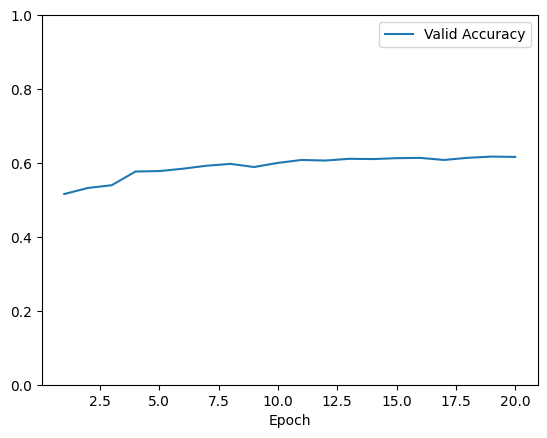
\includegraphics[width=0.8\textwidth]{"plots/logistic_regression-validation-accuracy-batch-16-lr-0.001-epochs-20-l2-0-opt-sgd.png"}
    \caption{Validation accuracy for $\eta = 0.001$}
    \label{2.1 0.001 Acc Plot}
\end{figure}

The test accuracies were 0.5577, 0.6200 and 0.6503 for $\eta = 0.1$, $\eta = 0.01$ and $\eta = 0.001$ respectively.\\
Looking at the plots, we can see that the best configuration, in terms of final valdiation accuracy, was $\eta = 0.01$.\\

\subsection{Question 2.2}

\subsubsection{Question 2.2 a)}
\paragraph{Answer} After running the code, the following plots were generated:
\begin{figure}[H]
    \centering
    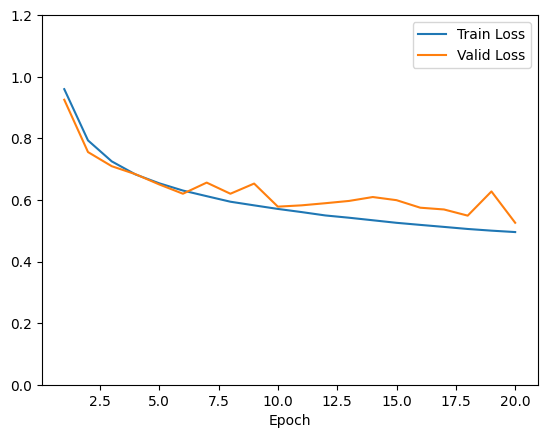
\includegraphics[width=0.8\textwidth]{"plots/mlp-training-loss-batch-16-lr-0.1-epochs-20-hidden-200-dropout-0.0-l2-0-layers-2-act-relu-opt-sgd.png"}
    \caption{Training and validation loss for batch size of 16}
    \label{2.2a batch size 16}
\end{figure}

\begin{figure}[H]
    \centering
    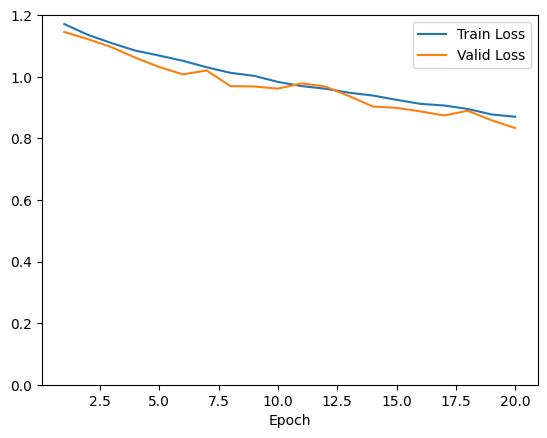
\includegraphics[width=0.8\textwidth]{"plots/mlp-training-loss-batch-1024-lr-0.1-epochs-20-hidden-200-dropout-0.0-l2-0-layers-2-act-relu-opt-sgd.png"}
    \caption{Training and validation loss for batch size of 1024}
    \label{2.2a batch size 1024}
\end{figure}

This exercise explores the trade-off between train time and performance when using different batch sizes. When training with smaller batch sizes, the model updates weights more frequently,
since each update is working with less data each time, and thus, takes more time to train when comparing to a bigger batch size. However, this frequent updating for smaller batch sizes can 
provide a regularizing effect avoiding overfitting. When compared to larger batch sizes, smaller batch sizes are more noisy, since they are more sensitive to the data they are working with. This noise can be positive, since it can help the model
to avoid converging to a local minimum and, that way, impoves the chances of finding the global minimum. On the other hand, the noise can also be negative, since it can lead to a slower convergence. On a overall note, smaller batch sizes often lead to a better 
model generalization and accuracy, despite taking more time to train. This comment can be supported by the plots above, where we can see that the model with batch size 16 has a better performance than the one with batch size 1024.

The best test accuracy was 0.7788 for batch size 16.

\subsubsection{Question 2.2 b)}
\paragraph{Answer} After running the code, the best and worst configurations were for learning rates of 0.1 and 1, respectively:

\begin{figure}[H]
    \centering
    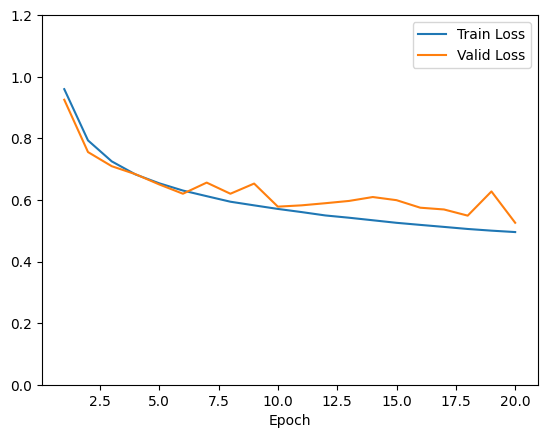
\includegraphics[width=0.8\textwidth]{"plots/mlp-training-loss-batch-16-lr-0.1-epochs-20-hidden-200-dropout-0.0-l2-0-layers-2-act-relu-opt-sgd.png"}
    \caption{Training and validation loss for learning rate of 0.1}
    \label{2.2b learning rate 0.1}
\end{figure}

\begin{figure}[H]
    \centering
    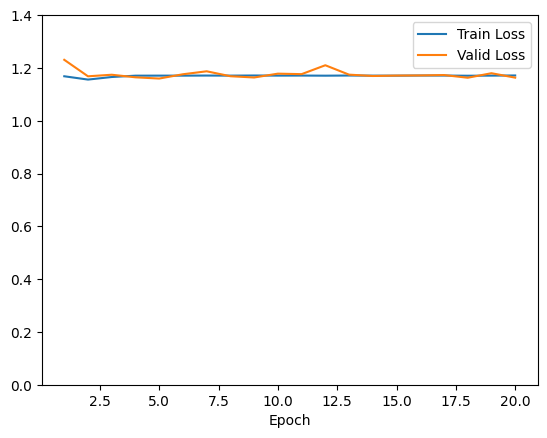
\includegraphics[width=0.8\textwidth]{"plots/mlp-training-loss-batch-16-lr-1.0-epochs-20-hidden-200-dropout-0.0-l2-0-layers-2-act-relu-opt-sgd.png"}
    \caption{Training and validation loss for learning rate of 1}
    \label{2.2b learning rate 1}
\end{figure}

This exercise explores the trade-off between a high and low learning rate. When using a high learning rate, the model converges faster, since it is taking bigger steps towards the minimum. 
However, this can lead to problems, since the model can overshoot the minimum and diverge. On the other hand, when using a low learning rate, the model takes smaller steps towards 
the minimum and thus, it takes more time to converge. This can be a good thing, since it can avoid overshooting the minimum and diverging. Important to note, that for a very low learning rate,
the model can get stuck in a local minimum, not achieving the best possible accuracy. For our specific case, the model with learning rate 1 didn't manage to converge, since it was taking steps too big and
overshooting the minimum, as we can see in the Figure \ref{2.2b learning rate 1}. For the learning rates 0.01 and 0.001, since the convergence is slower, 
the model was not able to reach a good accuracy in 20 epochs. The best test accuracy was 0.7788 for learning rate 0.1, wich offered a good balance between convergence speed and accuracy.

\subsubsection{Question 2.2 c)}
\paragraph{Answer} After running the code, the best configuration was for the model with a dropout probability of 0.2 and the worst one was for the default model.

\begin{figure}[H]
    \centering
    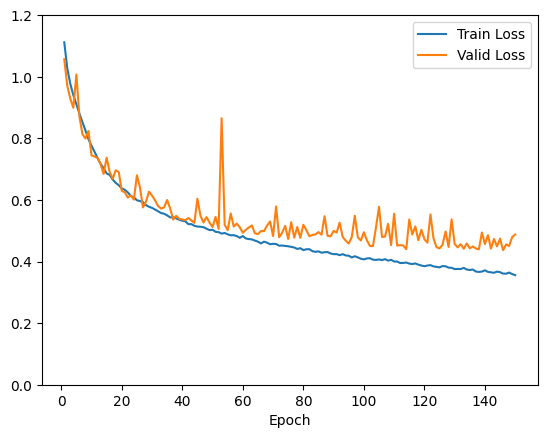
\includegraphics[width=0.8\textwidth]{"plots/mlp-training-loss-batch-256-lr-0.1-epochs-150-hidden-200-dropout-0.0-l2-0-layers-2-act-relu-opt-sgd.png"}
    \caption{Training and validation loss for default model}
    \label{2.2c default model}
\end{figure}

\begin{figure}[H]
    \centering
    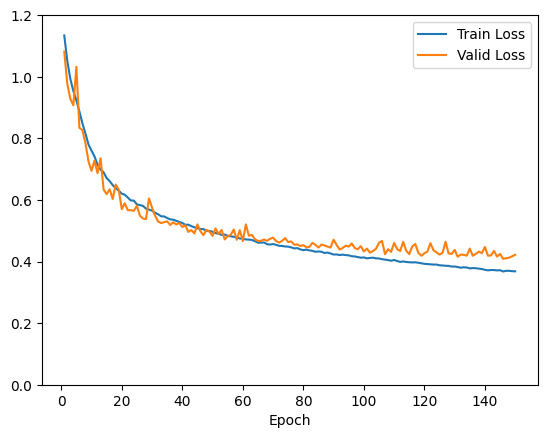
\includegraphics[width=0.8\textwidth]{"plots/mlp-training-loss-batch-256-lr-0.1-epochs-150-hidden-200-dropout-0.2-l2-0-layers-2-act-relu-opt-sgd.png"}
    \caption{Training and validation loss for model with dropout of 0.2}
    \label{2.2c dropout 0.2}
\end{figure}

In this exercise, we explore two different techniques to avoid overfitting. The base model, with no L2 regularization or dropout, 
suffered from overfitting, as we can see in the Figure \ref{2.2c default model}. To avoid this, we started with L2 regularization,
which adds a penalty term to the loss function, forcing the model to learn smaller weights, encouraging the model to find simpler solutions and,
that way, reducing the impact of noisy or irrelevant features. We also tested dropout, which is a technique that randomly drops a proportion of 
the network's nodes during each training epoch, forcing the network to avoid relying too heavily on any one feature. Both techniques were able to
reduce the overfitting, but the model with dropout of 0.2 was the one that achieved the best test accuracy, with an accuracy of 0.8034.


\section{Question 3}

\subsection{Question 3.1}
\subsubsection{Question 3.1 a)}
\paragraph{Answer}

To demonstrate that the specified Boolean function cannot be computed by a single perceptron, let's consider a simple case where \( D = 2 \), \( A = -1 \), and \( B = 1 \). The function \( f \) is defined as:

\[
f(x) = 
\begin{cases} 
1 & \text{if } \sum_{i=1}^{D} x_i \in [-1, 1], \\
-1 & \text{otherwise}
\end{cases}
\]

In this setup:

\begin{itemize}
    \item For \( x = (+1, +1) \), the sum \( \sum x_i = 2 \). Since 2 is not in the range [-1, 1], \( f(x) = -1 \).
    \item For \( x = (-1, -1) \), the sum \( \sum x_i = -2 \). Since -2 is also not in the range [-1, 1], \( f(x) = -1 \).
    \item For \( x = (-1, +1) \) or \( x = (+1, -1) \), the sum \( \sum x_i = 0 \). This falls within the range [-1, 1], so \( f(x) = 1 \) for these inputs.
\end{itemize}

The visual representation of the points can be seen in Figure \ref{3a Plot}. The red points represent the inputs that should be classified as \( +1 \) and the blue points represent the inputs that should be classified as \( -1 \).

The critical point here is that a single perceptron is fundamentally a linear classifier, which means it can only separate data points using a straight line in the feature space. However, in this example, there is no straight line that can separate these points accordingly in a 2D space, to satisfy the function \( f \).

This example thus serves as a counter-example proving that the given function cannot generally be computed with a single perceptron, as it requires a non-linear decision boundary which a single perceptron cannot provide. 

\begin{figure}[H]
    \centering
    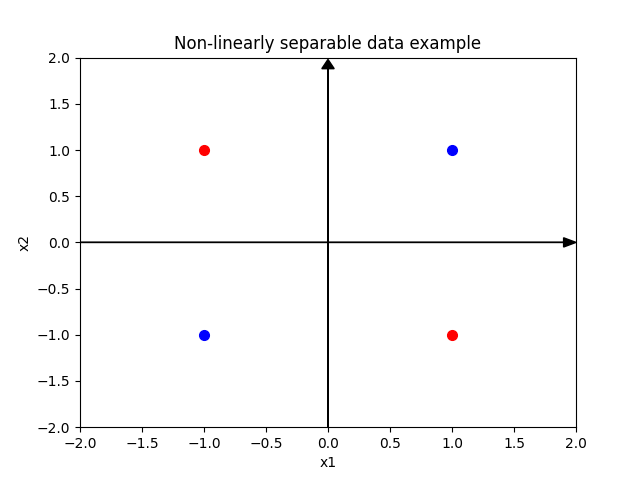
\includegraphics[width=0.8\textwidth]{"plots/3a.png"}
    \caption{Classification of points using the function \( f \)}
    \label{3a Plot}
\end{figure}
\subsubsection{Question 3.1 b)}
\subsubsection{Question 3.1 c)}

\end{document}
